\section{ Visualizing the data}


\begin{figure}[H]
    \centering
    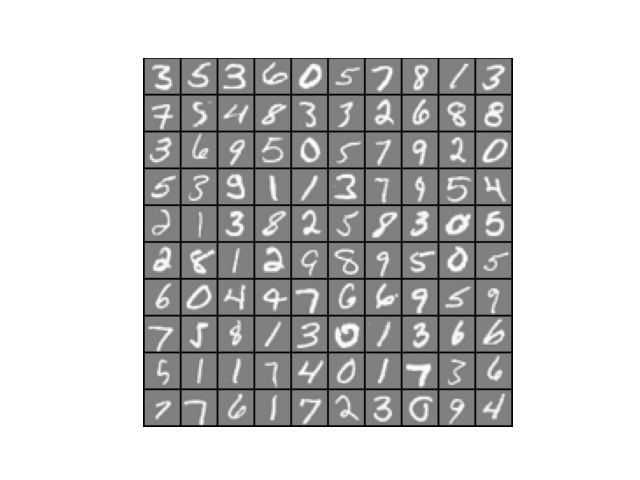
\includegraphics[width=0.75\linewidth]{figure/datas.png}
    \label{fig:placeholder}
\end{figure}

\subsection{Prediction by a neural network}
\subsection{ Model representation}
\subsection{Feedforward Propagation and Prediction}

\begin{lstlisting}
import numpy as np

from sigmoid import sigmoid

def predictNeuralNetwork(Theta1, Theta2, X):
    """ outputs the predicted label of X given the
    trained weights of a neural network (Theta1, Theta2)
    """

# Useful values
    m, _ = X.shape
    num_labels, _ = Theta2.shape

# ====================== YOUR CODE HERE ====================

    a1 = X

    z2 = a1 @ Theta1.T
    a2 = sigmoid(z2)
    a2 =  np.column_stack((np.ones((m,1)), a2))

    z3 = a2 @ Theta2.T
    a3 = sigmoid(z3)

    p = np.argmax(a3, axis=1)

# =================================================
    
    return p

\end{lstlisting}

\section{Learning a classifier with a neural Network}

\subsection{Feedforward and cost function}


\begin{lstlisting}
import numpy as np

from sigmoid import sigmoid
from sigmoidGradient import sigmoidGradient


def nnCostFunction(nn_params, input_layer_size, hidden_layer_size, num_labels, X, y, Lambda):

    theta1 = nn_params[0:(hidden_layer_size*(input_layer_size+1))].reshape((input_layer_size+1),hidden_layer_size).T
    theta2 = nn_params[(hidden_layer_size*(input_layer_size+1)):].reshape((hidden_layer_size+1),num_labels).T

# Setup some useful variables
    m, _ = X.shape

# You need to return the following variables correctly 
    X = np.column_stack((np.ones((m, 1)), X))
    z2 = X.dot(theta1.T)
    a2 = sigmoid(z2)
    a2 = np.column_stack((np.ones((m, 1)), a2))
    z3 = a2 @ theta2.T
    a3 = sigmoid(z3) 
    # h = np.argmax(a3, axis=1)
    y_train = np.zeros((m, num_labels))
    y_train[np.arange(m), y.flatten()] = 1

    J = 1/m * np.sum(-y_train*np.log(a3) - (1-y_train)*np.log(1-a3))


\end{lstlisting}

\begin{itemize}
    \item Output:
\end{itemize}

\begin{figure}[H]
    \centering
    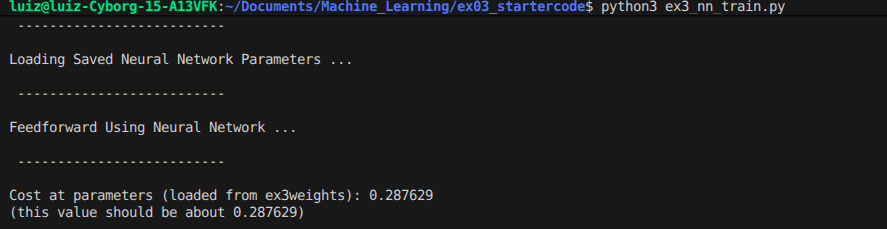
\includegraphics[width=0.75\linewidth]{figure/5.1.png}
    \label{fig:placeholder}
\end{figure}


\subsection{Regularized cost function}


\begin{lstlisting}
    ...
    J = 1/m * np.sum(-y_train*np.log(a3) - (1-y_train)*np.log(1-a3))

     # Cost regularisation
    reg = Lambda/(2*m) * (np.sum(theta1[:,1:]**2) + np.sum(theta2[:,1:]**2))
    J = J + reg

\end{lstlisting}

\begin{itemize}
    \item Output:
\end{itemize}

\begin{figure}[H]
    \centering
    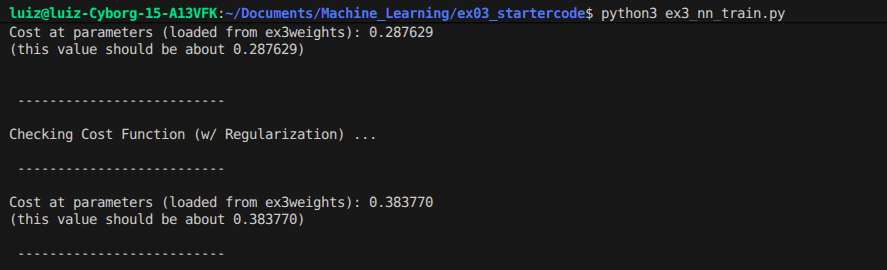
\includegraphics[width=0.75\linewidth]{figure/5.2.png}
    \label{fig:placeholder}
\end{figure}


\subsection{Backpropagation}
\subsubsection{Sigmoid gradient}

\begin{lstlisting}
from sigmoid import sigmoid

def sigmoidGradient(z):
    """computes the gradient of the sigmoid function
    evaluated at z. This should work regardless if z is a matrix or a
    vector. In particular, if z is a vector or matrix, you should return
    the gradient for each element."""

# ====================== YOUR CODE HERE ======================
# Instructions: Compute the gradient of the sigmoid function evaluated at
#               each value of z (z can be a matrix, vector or scalar).

    g = sigmoid(z) * (1 - sigmoid(z))

# =============================================================

    return g

\end{lstlisting}

\begin{itemize}
    \item Output:
\end{itemize}

\begin{figure}[H]
    \centering
    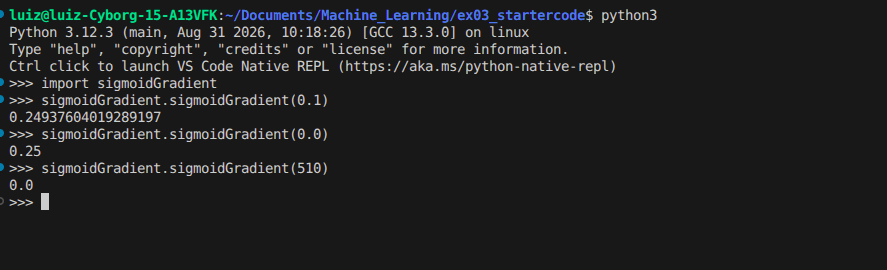
\includegraphics[width=0.75\linewidth]{figure/531.png}
    \label{fig:placeholder}
\end{figure}

\subsubsection{ Random initialization}

\begin{lstlisting}
import numpy as np

def randInitializeWeights(L_in, L_out):
    """randomly initializes the weights of a layer with L_in incoming connections and L_out outgoing
      connections.

      Note that W should be set to a matrix of size(L_out, 1 + L_in) as the 1st column of W handles the "bias" terms
    """

    # ====================== YOUR CODE HERE ===================================
    # Instructions: Initialize W randomly so that we break the symmetry while
    #               training the neural network.
    #
    # Note: The first row of W corresponds to the parameters for the bias units
    #

    epsilon_init = 0.12
    W = np.random.rand(L_out, 1+L_in) * 2 * epsilon_init - epsilon_init


    # =====================================================

    return W


\end{lstlisting}

\subsubsection{The backpropagation algorithm}

\subsubsection{Gradient checking}

\begin{itemize}
    \item Output:
\end{itemize}

\begin{figure}[H]
    \centering
    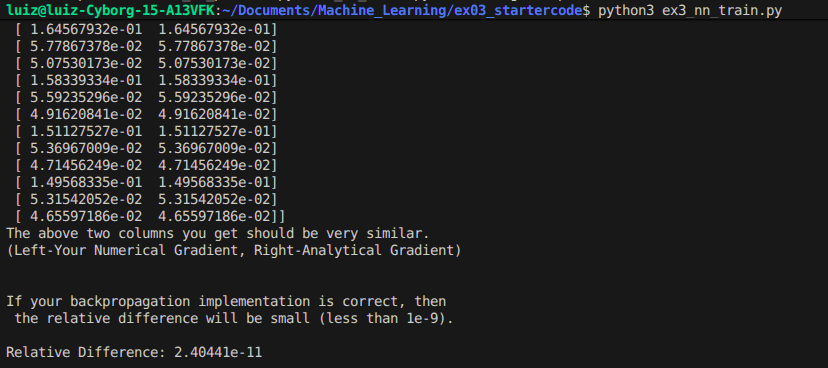
\includegraphics[width=0.75\linewidth]{figure/checking.png}
    \label{fig:placeholder}
\end{figure}

The relative difference between the analytical and numerical gradients is very small, which indicates that the backpropagation implementation is correct.

\subsubsection{ Regularized Neural Networks}

\subsubsection{Learning parameters using fmin\_cg}

\begin{figure}[H]
    \centering
    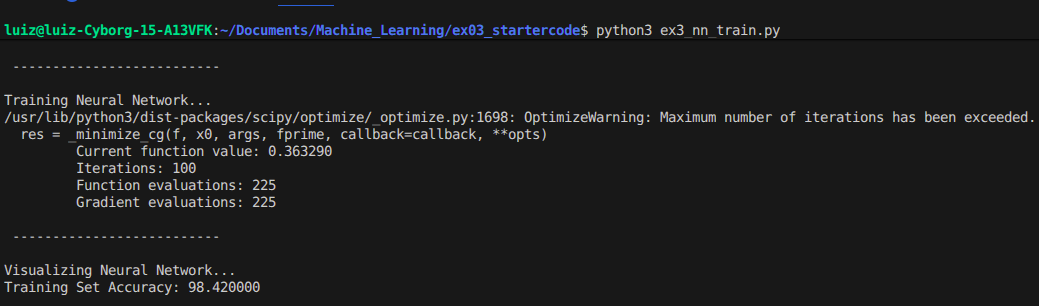
\includegraphics[width=0.75\linewidth]{figure/fmin.png}
    \label{fig:placeholder}
\end{figure}

\subsection{Visualising the hidden layer}

\begin{figure}[H]
    \centering
    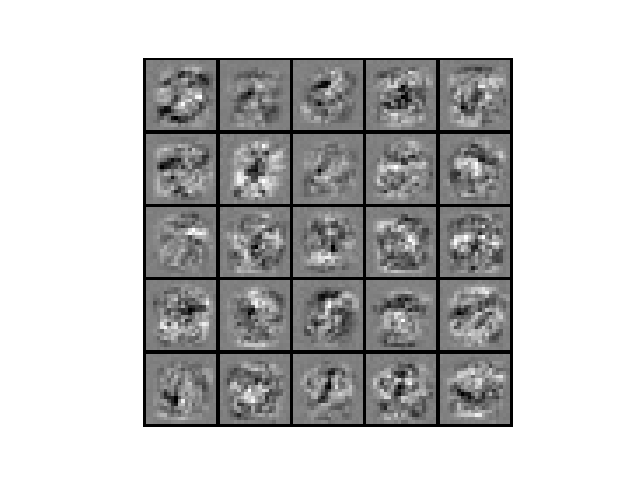
\includegraphics[width=0.75\linewidth]{figure/hiddenLayer.png}
    \label{fig:placeholder}
\end{figure}

\subsection{Final analysis}

\begin{itemize}
    \item Results if $\lambda = 0.1$ and $maxIter = 150$:
\end{itemize}

\begin{figure}[H]
    \centering
    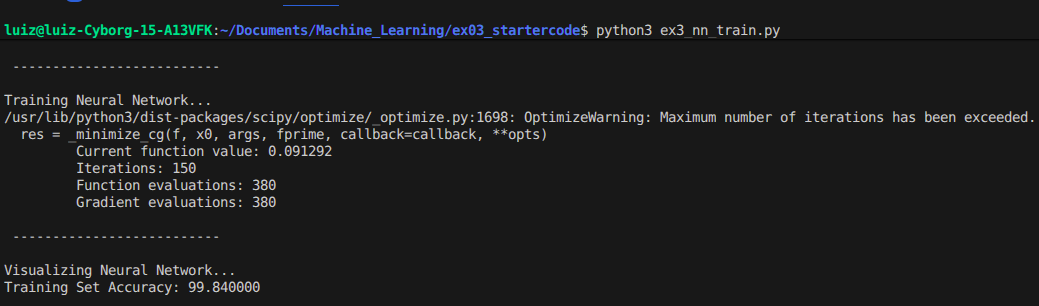
\includegraphics[width=0.75\linewidth]{figure/overTrain.png}
    \label{fig:placeholder}
\end{figure}

\begin{itemize}
    \item Displaying the hidden layers:
\end{itemize}

\begin{figure}[H]
    \centering
    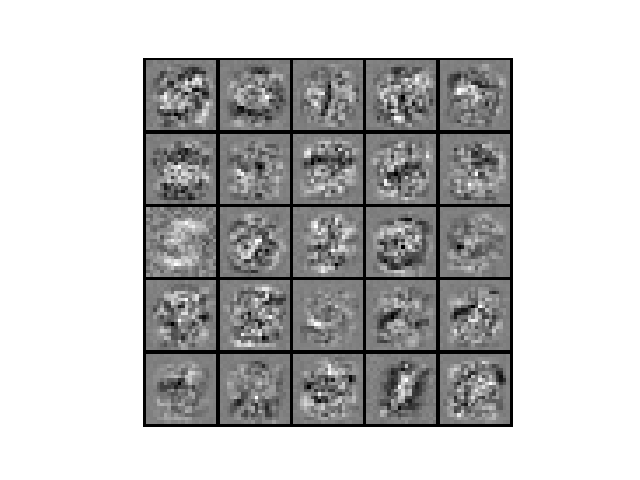
\includegraphics[width=0.75\linewidth]{figure/overTraining.png}
    \label{fig:placeholder}
\end{figure}

\section{Some questions}

\begin{itemize}
    \item Décrivez l’approche basée sur les réseaux de neurones. Quelle modélisation est retenue? Quels sont
les paramètres à apprendre?
    \subitem The neural network is an approach that allows us to solve complex real world problems. By adding hidden layers, we can build non-linear decision boundaries of various shapes. The parameters to learn are the weights connecting the neurons between each layer, usually defined as Theta matrices.
    \item Quelle est la fonction de coût? Quelles modifications sont effectuées par rapport à celle utilisée en
TP2?
    \subitem The cost function is a mathematical metric that measures the difference between the computed predictions and the actual expected values. It helps us track if the network is training correctly, because if the cost grows or stays constant after each iteration, something is wrong. Here, we are dealing with a multi-class problem, so the cost function uses a double sum to compute the error across all output classes for each example. In contrast, TP2 was a binary classification problem, so we only needed a single sum.
  
\end{itemize}